Метод двухкристальной дифрактометрии широко распространен для исследования пьезоэлектрических свойств \cite{piezo51} - \cite{piezo54}.
Для того, чтобы зафиксировать смещение пика двухкристальной КДО, необходимо проснять кривую дифракционного отражения
до и после приложенного напряжения (рис. \ref{ris:piezo_classic}).
\begin{figure}[H]
  \centering
  \subfloat[]{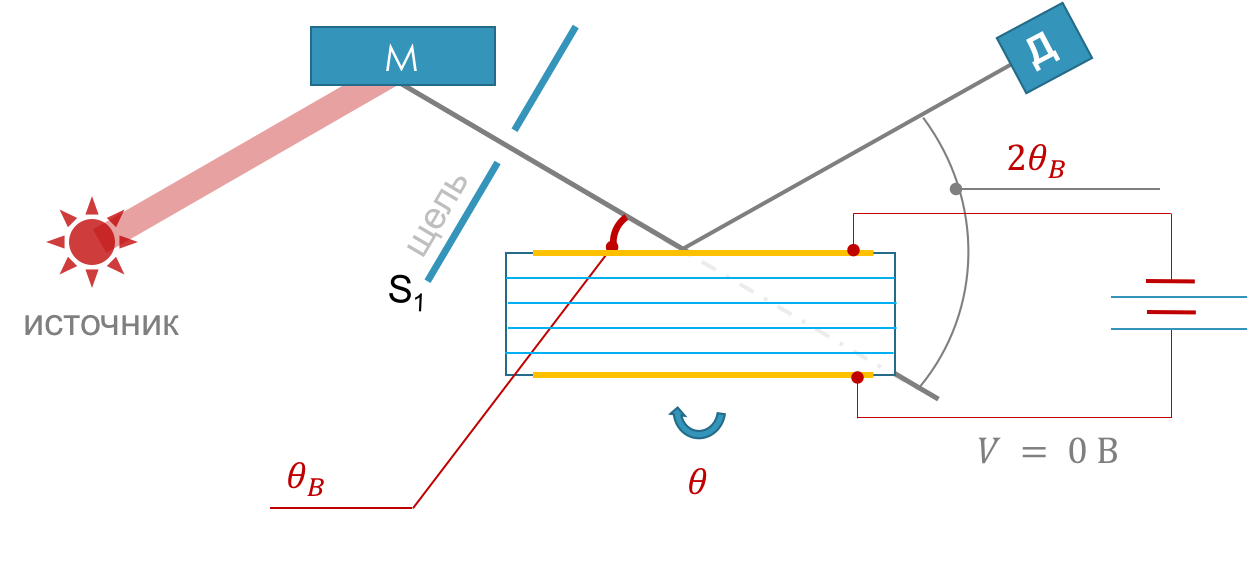
\includegraphics[width=0.33\textwidth]{images/piezo_classic_1.png}\label{ris:piezo_classic_1}}
  \hfill
  \subfloat[]{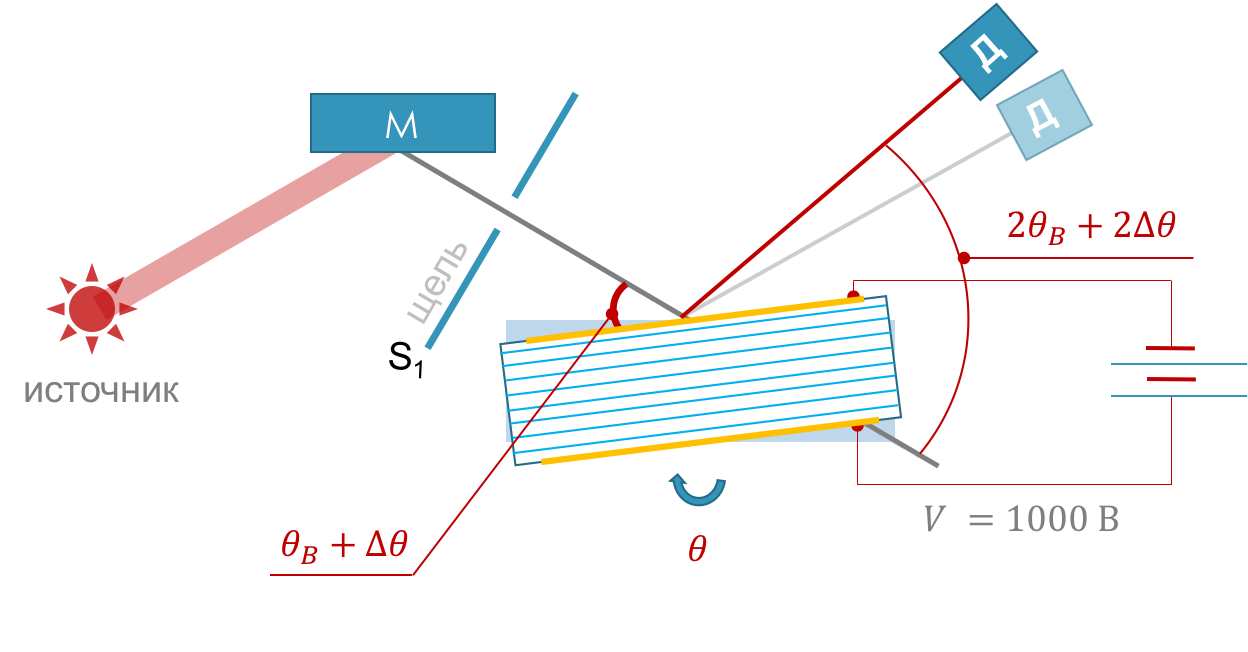
\includegraphics[width=0.33\textwidth]{images/piezo_classic_2.png}\label{ris:piezo_classic_2}}
  \hfill
  \subfloat[]{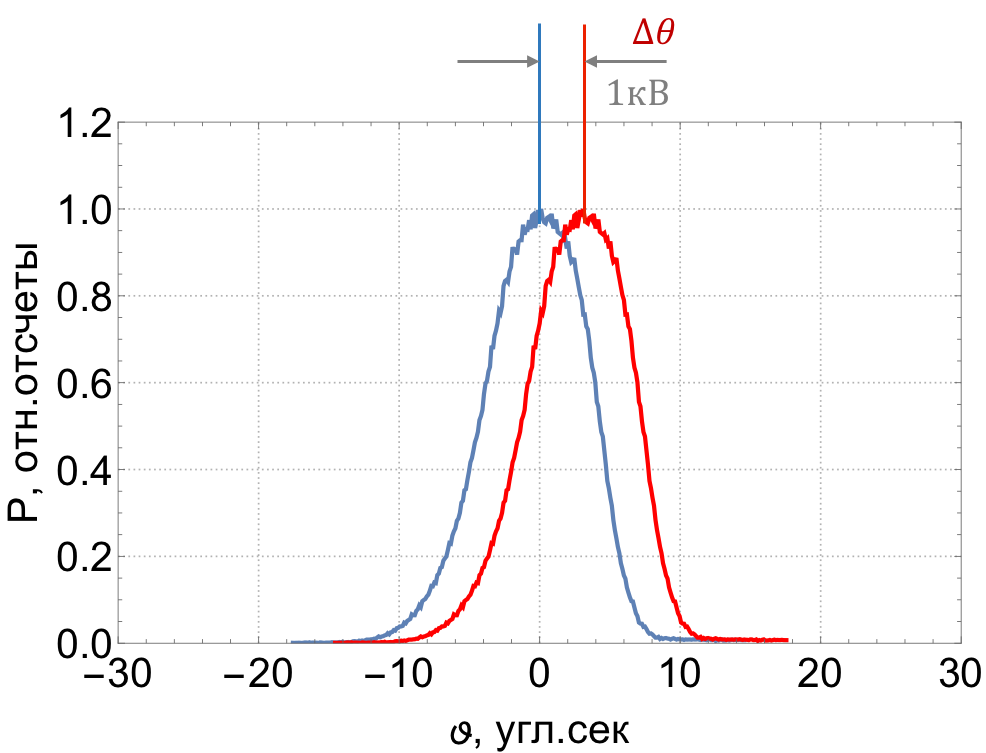
\includegraphics[width=0.2\textwidth]{images/piezo_classic_3.png}\label{ris:piezo_classic_3}}

  \caption{Схематичное представление методики измерения сдвига брэгговского максимума. Cхема
  (a) в отсутствии электрического поля, (b)  под действием электрического поля проиходит изменение угла
  Брэгга, (c) изменеие положения максимума КДО}
  \label{ris:piezo_classic}
\end{figure}
  Такой метод не позволяет отследить динамику в момент приложения электрического поля,
  т.к. время за которое получается КДО на лабораторном источнике составляет десятки секунд.
